%!TEX root = ../main.tex
 \section{自然言語処理の実践}

 本節では,ニューラルネットワーク用フレームワークの Chainer を用いて自然言語を扱う方法を学ぶ.

 まず最初に,リカレントニューラルネットワークを用いた言語モデルの学習を行い,動作を確認する.その後,エンコーダー・デコーダモデルを用いた英日翻訳機を作成し,学習及び動作の確認を行う.

  \subsection{言語モデルの作成}
 まずはじめに,RNNを用いて日本語の言語モデルを学習する.「言語モデル」の詳しい説明は理論編を参照すること.

 なにはともあれまずはサンプルを実行してみよう.実験で使用するソースコードはサーバーのホームディレクトリに\verb+dl_exp_nlp.tar.gz+ という名前で配置されている.
  \begin{lstlisting}[basicstyle=\ttfamily\footnotesize, frame=single]
   $tar xzvf dl_exp_nlp.tar.gz
   $cd dl_exp_nlp
   $python language_model_rnn_train.py
  \end{lstlisting}
学習には10分前後かかるため,その間にプログラムの解説を行う.学習データは,datasetディレクトリ内の\verb+data_1000.txt+ を使用している.一行毎に,英文とそれに対応する日本語文がタブ文字で区切られて記入されている.また,それぞれの文は半角スペースで単語に区切られている.
\begin{itemize}
\item 学習データは,「田中コーパス」 (\url{http://www.edrdg.org/wiki/index.php/Tanaka_Corpus}) を加工したものである.
\item 「コーパス」とは,主に研究目的のため,自然言語のデータを体系的に収集し,構造化したデータのことを指す.
\item \verb+data_full.txt+ は田中コーパスの全てのデータであり,\verb+data_100.txt+ ,\verb+data_1000.txt+ はコーパスの中からそれぞれ100文,1000文を抜き出したものになっている.
\end{itemize}
学習データのパースを行っている\verb+sentence_data.py+ を見てみよう.自然言語処理の分野ではしばしば単語を「ID」で管理する.今回のプログラムでも,コーパス中の各単語にIDを割り振っている.日本語については\verb+SentenceData+ クラスの\verb+japanese_word_id()+ メソッドで「単語文字列$\rightarrow$単語ID」,\verb+japanese_word()+ メソッドで「単語ID$\rightarrow$単語文字列」の変換を行えるようになっている.また,\verb+japanese_sentence_data()+ メソッドはインデックスを与えると対応する文章データを返すが,これは「単語IDのリスト」という形式であることに注意する.なお,文の終端を表す EOS (End of Sentence) という概念が存在する.今回は EOS のIDを0と定義した.

  \begin{figure}[htb]
   \centering
   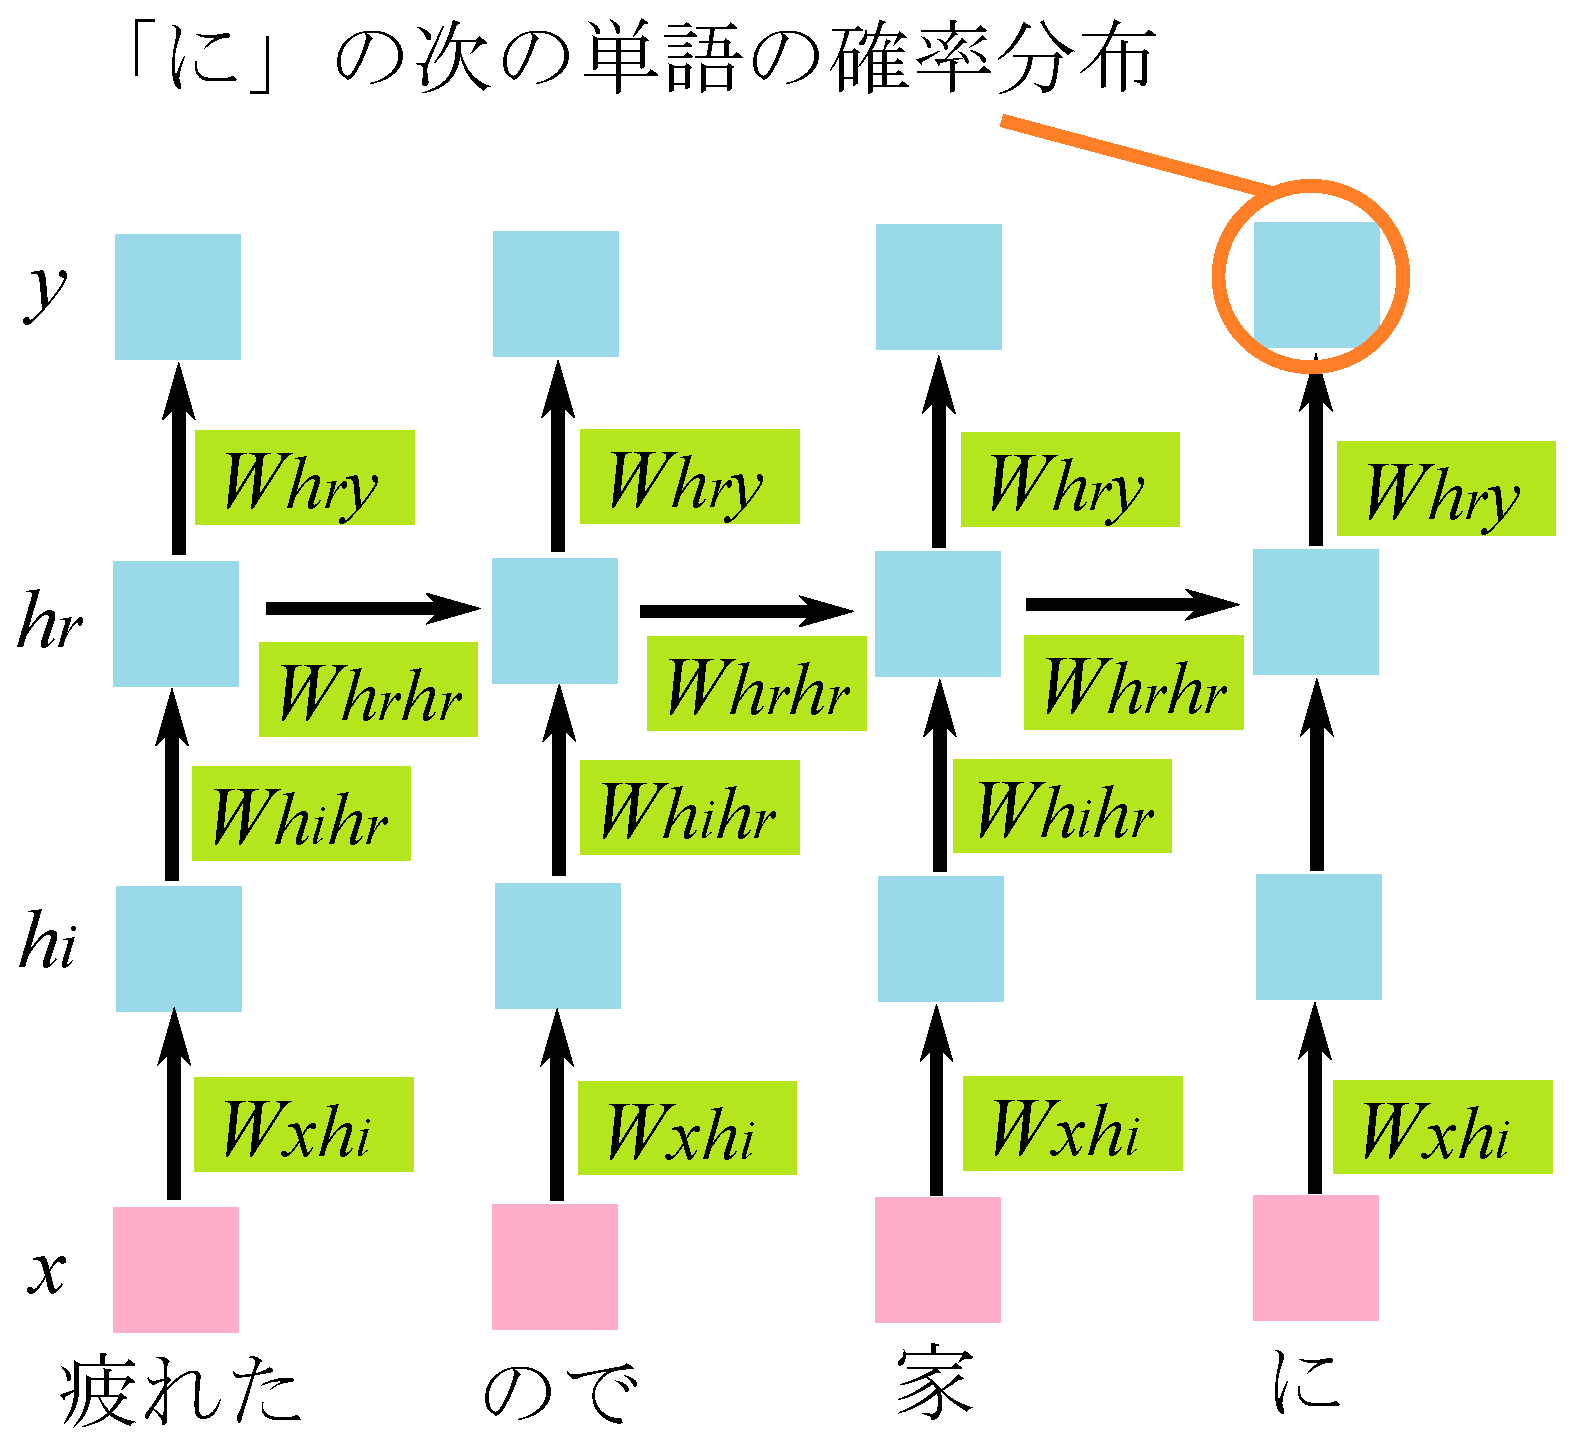
\includegraphics[width=80mm]{images/TsuruokaLab/langmodel.eps}
   \caption{RNN を用いた言語モデル}
   \label{fig:langmodel}
  \end{figure}

次に\verb+language_model_rnn.py+ を読む.\verb+LanguageModel+ というクラスが定義されており,\verb+chainer.Chain+ クラスを継承している.\verb+chainer.Chain+ はニューラルネットワークのモデルを表現するためのクラスであり,ネットワークのパラメータを\verb+chainer.Chain+ の\verb+__init__+ に渡している.今回用いるのは図\ref{fig:langmodel}に示すネットワークである.$x$は単語IDを表現するベクトルで,語彙数に等しい次元を持ち,単語IDに対応する位置の要素のみ1で,他の要素は0になっている.このようなベクトルを one hot vector と呼ぶ.本来ならばニューラルネットワークの入力としてはこの one hot vector を用いなければならないが,Chainer には one hot vector を扱うための\verb+EmbedID+ というクラスが存在する.このクラスは,入力に one hot vector の代わりに単一の整数を取ることができ,指定した整数の位置が1となる one hot vector として扱ってくれる.今回は$W_{xh_i}$が\verb+EmbedID+ になる.$W_{xh_i}$は,単語IDに対応する$h_i$の組が横に並んだ行列と見ることもできる.\verb+Linear+ クラスは単なる行列である.\verb+EmbedID+ や\verb+Linear+ には初期化時に入力の次元と出力の次元を渡す必要がある.

また,今回はリカレントニューラルネットワークとして,隠れ層$h_r$の値を保存する必要があるため,メンバとして$h_r$の値を持っており,\verb+reset_state()+ メソッドで初期化できるようにしている.\verb+__call__+ により,単語IDを入力として受け取りネットワークの出力を返す.出力は,語彙数の次元を持ち,各単語IDに対応する位置の値が,その単語の出現確率を示している.
\begin{itembox}[l]{softmax}
より正確には,出力ベクトルに softmax と呼ばれる処理を行うことで,ベクトルの要素を確率に変換する.
\end{itembox}


\verb+language_model_rnn_train.py+ で実際に学習を行っている.学習データ全体を一周すると「1 epoch」となり,今回はデフォルトでは 10 epochs の学習を行う.学習結果は 1 epoch 毎に,\verb+trained_model+ ディレクトリ以下に保存される.

さて,そろそろ学習が終わっただろうか.学習が終了したら,\verb+language_model_rnn_test.py+ を実行することで,学習した言語モデルをテストすることができる.
  \begin{lstlisting}[basicstyle=\ttfamily\footnotesize, frame=single]
   $python language_model_rnn_test.py
  \end{lstlisting}
として実行し,最初の単語,例えば「私」と入力すると,2単語目に来る確率が最も高い単語が出力される.さらに,「入力した1単語目,推定された2単語目」という単語列から,最も確率の高い3単語目が続けて出力され,文の終端である EOS が出力されるまで,再帰的に推定を行う.入力には半角スペースで区切った複数単語を入れることもでき,「私 は ここ」と入力した場合は,最も確率の高い4単語目から推定が行われる.
 \begin{practice}
   適当な単語または単語列を入力し,入力によって出力が変化すること,ある程度「日本語らしい」文章になることを確認せよ.
 \end{practice}
 \newpage

  \subsection{Long Short-Term Memory (LSTM)}
 理論編で学んだように,単純な RNN で精度の良い学習を行うのは難しく,LSTM や GRU 等の改良された構造が用いられることが多い.ここでは LSTM を使用して先程と同様に言語モデルの学習を行う.

  \begin{figure}[htb]
   \centering
   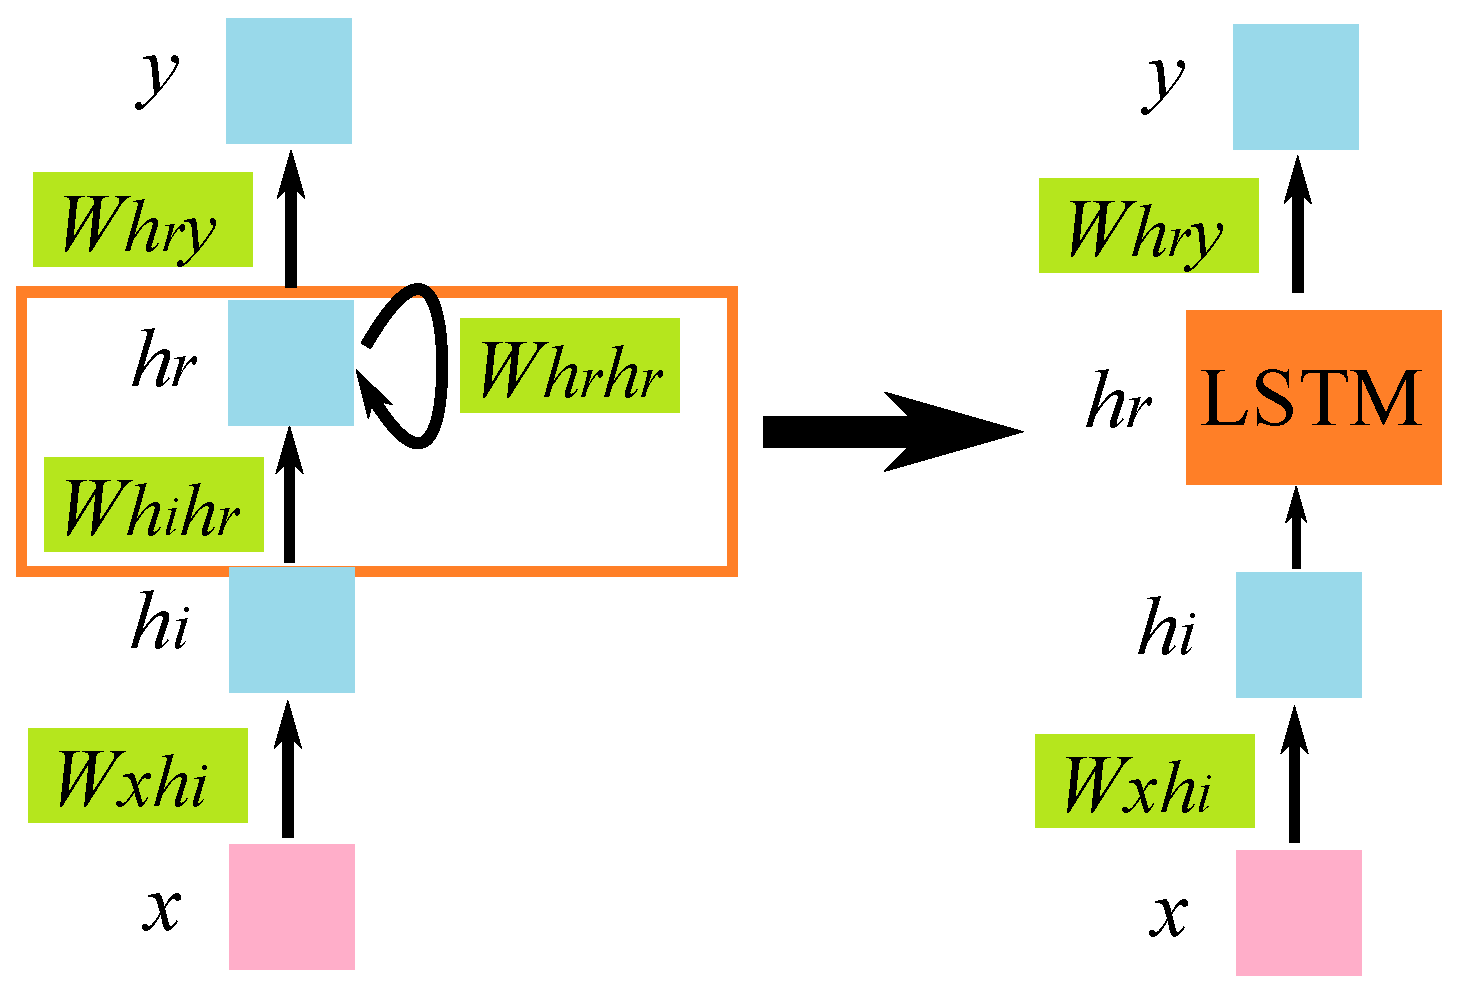
\includegraphics[width=80mm]{images/TsuruokaLab/lstm.eps}
   \caption{ChainerのLSTMクラスによる RNN の置き換え}
   \label{fig:lstm}
  \end{figure}

 Chainer には既に LSTM のモデルが用意されている.図\ref{fig:lstm}に示すように,RNN 部分をまるごと置き換えるようになっており,隠れ層のデータも含まれている.\verb+language_model_lstm.py+ に,LSTM を用いて言語モデルの学習を行う例を示した.RNN を自分で実装したときとは異なり,\verb+reset_state()+ メソッドでは,\verb+chainer.links.LSTM+ の\verb+reset_state()+ メソッドを呼び出す様になっている.これは,隠れ層のデータは\verb+chainer.links.LSTM+ の内部に含まれているからである.さて,今回は\verb+LanguageModel+ クラスの\verb+__call__+ の実装をまだ行っていない.\verb+language_model_rnn.py+ も参考にしつつ,各自で実装してみよ.
 \begin{practice}
 \verb+language_model_lstm.py+ における\verb+LanguageModel+ クラスの\verb+__call__+ を実装し,実際に学習を行ってみよ.学習は\verb+language_model_lstm_train.py+ を実行することで行うことができる.学習が終了したら,\verb+language_model_lstm_test.py+ を実行し,動作を確認せよ.
 \end{practice}
 \begin{practice}
  \verb+language_model_lstm_train.py+ 及び\verb+language_model_lstm_test.py+ を書き換え,英語の言語モデルを学習し,動作を確認せよ.学習には時間がかかるため,学習中に次の章を読み進めておくと良い.
 \end{practice}

  \subsection{エンコーダー・デコーダモデル}
 次に,エンコーダー・デコーダモデルを用いた英日翻訳機の学習を行う.エンコーダー・デコーダモデルについては理論編を参照すること.LSTM を用いた英日翻訳の例を図\ref{fig:encdecexample}に示す.\verb+translator_model.py+ を読むと,このモデルが定義されている.注意点として,Chainer の\verb+LSTM+ クラスは隠れ層のデータを内部に保持している.今回は隠れ層のデータをエンコーダ用LSTMからデコーダ用LSTMに引き継ぐ必要があるため,\verb+LSTM+ クラスの代わりに\verb+StatelessLSTM+ クラスを用いた.\verb+StatelessLSTM+ は,隠れ層のデータを内部に持たず,外部に変数として保存して計算時に与えるようになっている.また理論編で学んだように,LSTMは隠れ層の他にメモリーセルと呼ばれる状態ベクトルも持つため,これも隠れ層と同様に変数として保存する必要がある.

  \begin{figure}[htb]
   \centering
   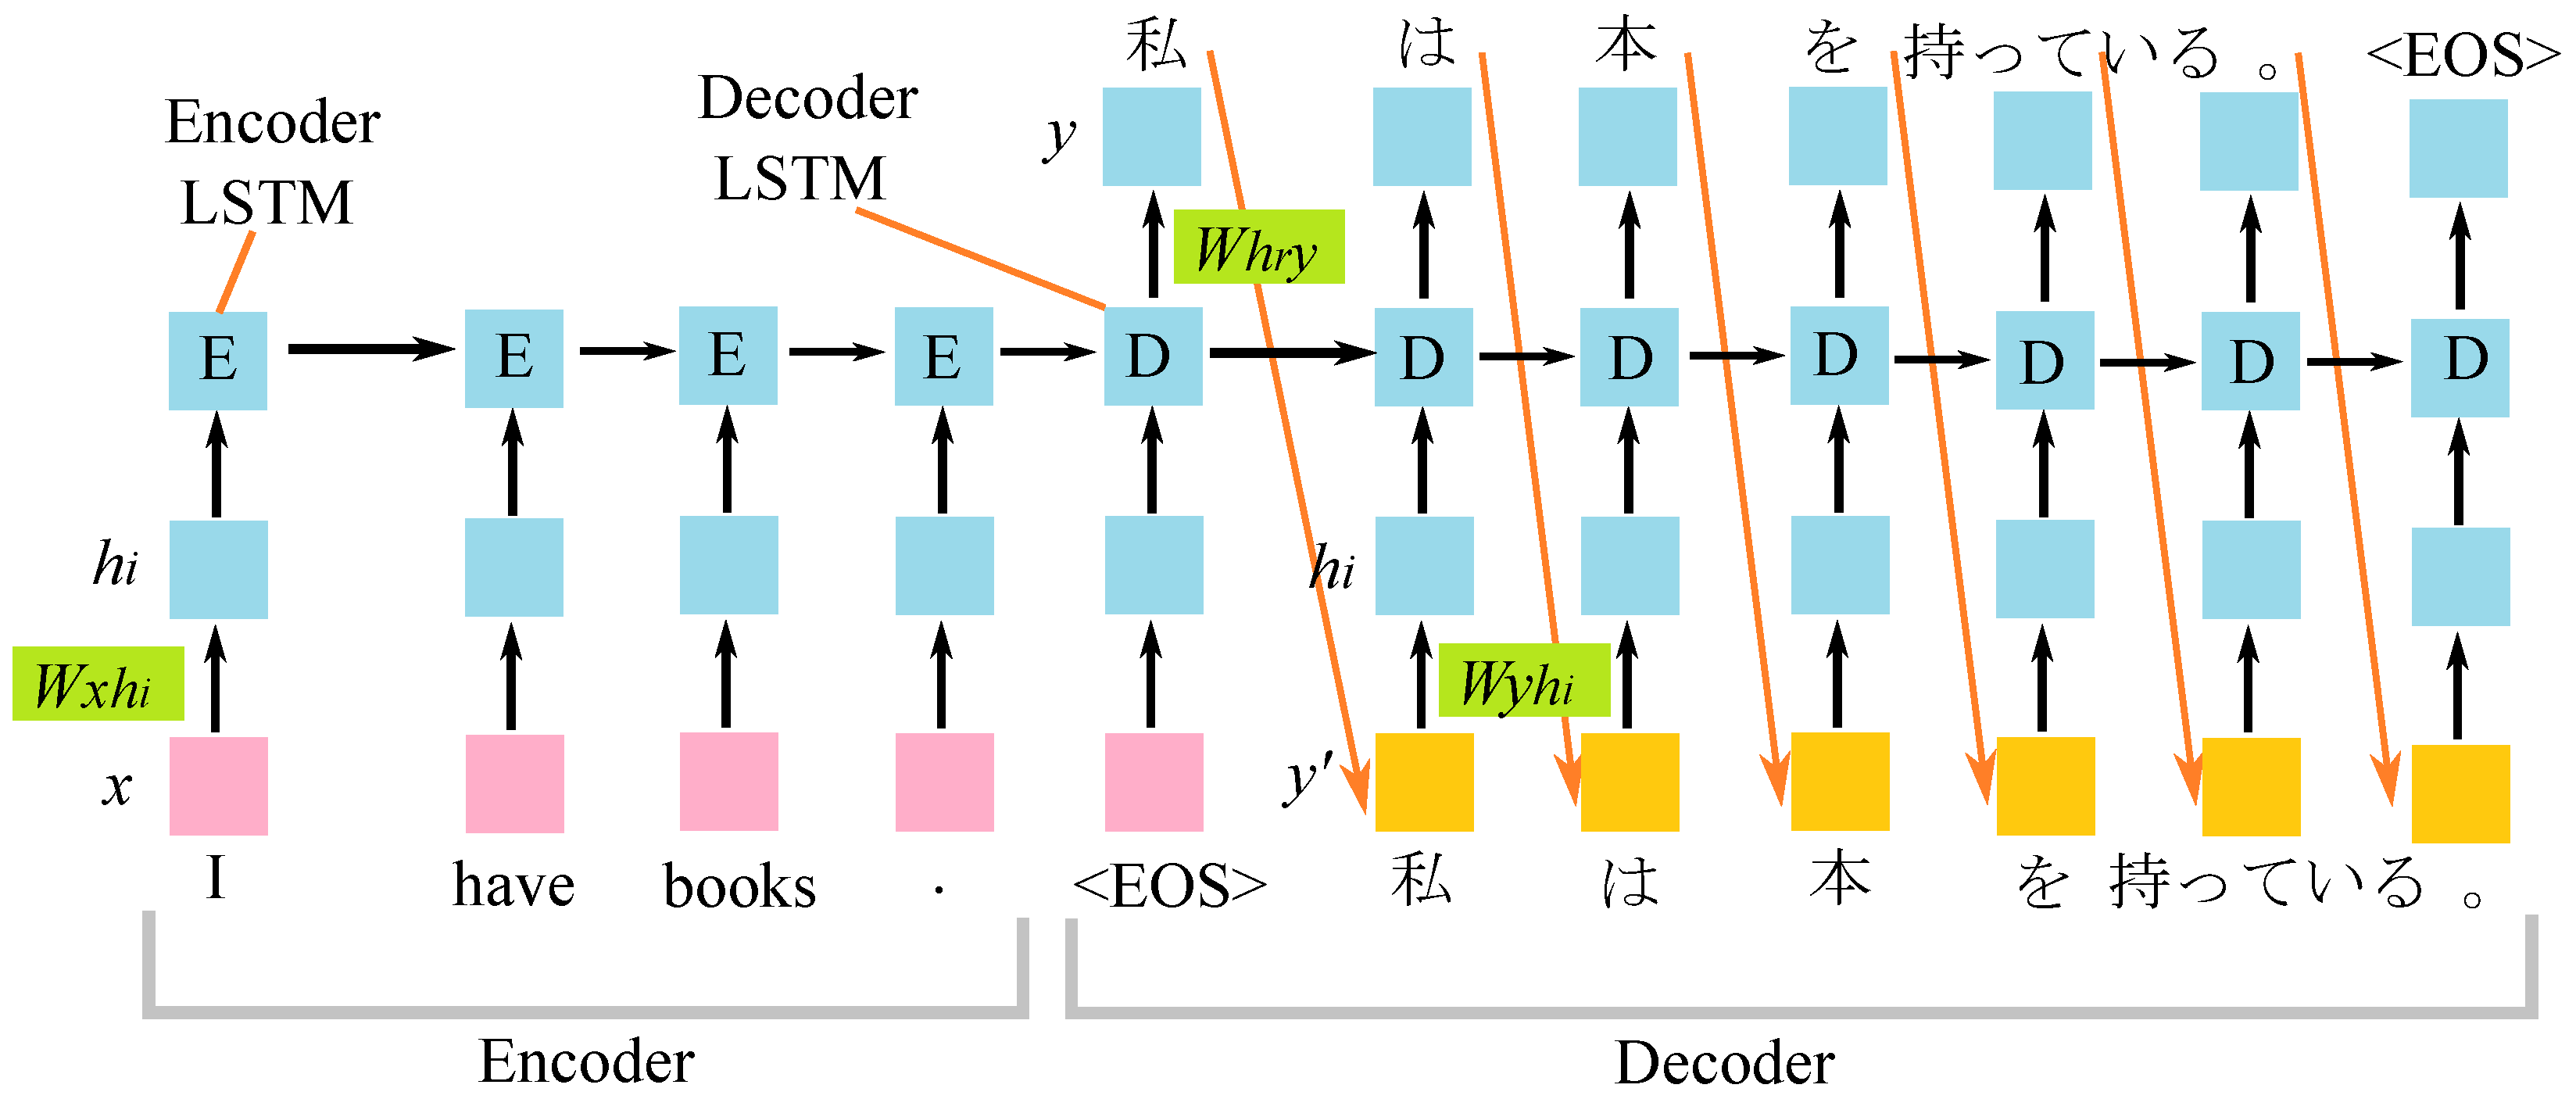
\includegraphics[width=130mm]{images/TsuruokaLab/encdecexample.eps}
   \caption{エンコーダー・デコーダモデルによる英日翻訳}
   \label{fig:encdecexample}
  \end{figure}

 \begin{practice}
  \verb+translator_model_train.py+ を実行し,翻訳モデルの学習を行ってみよ.学習している間に,\verb+translator_model.py+ 及び\verb+translator_model_train.py+ を読んで,ネットワークを定義している部分,エンコードやデコードを行う部分などを探してみよ.
 \end{practice}
 \begin{practice}
  学習が終了したら,\verb+translator_model_test.py+ を実行し,結果を確かめてみよ.入力の際は「I have a book .」のように,ピリオドも単語として区切るため,スペースを挟む必要があることに注意する.
 \end{practice}

大抵の場合,一見日本語のような文章ではあるが,翻訳結果としては間違った文章が出力されたと思われる.これは主に学習データの数が足りないためである.今回は1000文の学習データを用いて 10 epochs の学習を行ったが,この数では正確な翻訳は不可能である.\verb+traind_model/translator_full.model+ は,\verb+data_full.txt+ を用いて約15万文で 10 epochs の学習を行ったデータである.\verb+translator_model_test_full.py+ を実行することで,このデータを用いて翻訳を行うことができる.
 \begin{practice}
  \verb+translator_model_test_full.py+ を実行し,動作を確認せよ.
 \end{practice}

  \subsection{未知語対応}
 今までのプログラムで作成したモデルでは,コーパスに含まれない単語が入力された場合に対応できなかった.そこで,未知の単語が入力された場合でもある程度動作する仕組みを考える.簡単な例としては,未知の単語を共通の「\textless UNKNOWN\textgreater 」という単語に置き換えてしまうという手法が考えられる.この手法を動作させるには,学習の際に「\textless UNKNOWN\textgreater 」を含むデータセットが必要になる.そのため,データセットを読み込む際に変換を行う.変換方法の例としては
\begin{itemize}
\item 出現回数が一定回数以下の単語を全て「\textless UNKNOWN\textgreater 」に置き換える.
\item 各単語が初めて出現したときに「\textless UNKNOWN\textgreater 」に置き換える.
\end{itemize}
等が考えられる.「\textless UNKNOWN\textgreater 」を扱うための準備として,\verb+sentence_data.py+ に
  \begin{lstlisting}[basicstyle=\ttfamily\footnotesize, frame=single]
UNKNOWN_WORD_ID = 1
  \end{lstlisting}
を追記し,また単語の辞書作成部分は
  \begin{lstlisting}[basicstyle=\ttfamily\footnotesize, frame=single]
    self.en_word_to_id = {"<EOS>":EOS_ID, "<UNKNOWN>":UNKNOWN_WORD_ID}
    self.en_word_list = ["<EOS>", "<UNKNOWN>"]
    self.jp_word_to_id = {"<EOS>":EOS_ID, "<UNKNOWN>":UNKNOWN_WORD_ID}
    self.jp_word_list = ["<EOS>", "<UNKNOWN>"]
  \end{lstlisting}
とする.
 \begin{practice}
  \verb+sentence_data.py+ の\verb+__init__+ で学習データを読み込んでいる部分を書き換え,データセットに「\textless UNKNOWN\textgreater 」が含まれるようにせよ.
 \end{practice}
 \begin{practice}
  \verb+language_model_lstm_test.py+ や,\verb+translator_model_test.py+ を書き換え,未知の単語が入力された場合に「\textless UNKNOWN\textgreater 」に置き換えて,出力が得られるようにせよ.これをテストする場合は,前の課題で書き換えた\verb+sentence_data.py+ を用いて学習をやり直す必要があることに注意せよ.
 \end{practice}

  \subsection{発展課題}
余力のある人は,以下の発展課題に取り組んでみよ.
\begin{itemize}
\item いくつかの学習データをまとめて学習することで,主にGPUを使用する場合の学習効率を上げることができる.この手法を mini batch と呼ぶ.Chainer では入力データの次元を挙げることで簡単に mini batch 化が可能であるが,系列データはデータによってデータ長が異なるため,少々面倒である.Chainer には可変長データをバッチ化しやすくするために NStepLSTM というクラスがある.NStepLSTM の使い方を調べ,実験で用いたプログラムを mini batch 化せよ.
\item 今回は単語IDから特長ベクトル$h_i$を生成するための行列$W_{xh_i}$も同時に学習したが,各単語を表す特徴ベクトルを事前に学習することも可能である.学習済みのデータを公開している人も多いので,それらのデータを用いるように今回のプログラムを変更してみよ.Word embedding や, Word2Vec 等のキーワードで検索すると良い.
\item 配布したデータセットは,前述のように田中コーパス (\url{http://www.edrdg.org/wiki/index.php/Tanaka_Corpus}) を加工したものであるが,加工前のコーパスデータには,単語の原型などの追加データが存在する.それらのデータを上手く使うことで,学習の効率や精度を上げることができないか検討せよ.なお,今回英単語の切り分けには Stanford CoreNLP (\url{https://stanfordnlp.github.io/CoreNLP/}) を用いた.
\item ネットワークの構造を変更することで,より精度良く学習が行なえないか検討せよ.例えば,理論編で学んだ attention を導入してみよ.
\end{itemize}

  \subsection{自由課題のヒント}
\begin{itemize}
\item エンコーダー・デコーダモデルの用途は翻訳に限らず,系列データの入力から系列データを出力する一般のタスクに応用できる.例えば,長い文章を入力すると要点をまとめて短くしてくれるような要約タスクなどが考えられる.
\item RNN の入力や出力は単語(列)に限らない.例えば画像分野と組み合わせて,連続画像を入力としたり,画像から文章を生成する等の応用も考えられる.
\end{itemize}
